\documentclass[tikz,border=2pt]{standalone}
\usepackage{tikz}
\usetikzlibrary{calc}
\begin{document}
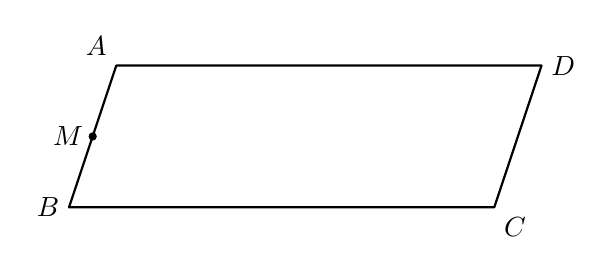
\begin{tikzpicture}[line cap=round,line join=round]
  % Parallelogram
  \coordinate (A) at (1.4,2.6);
  \coordinate (B) at (0.8,0.8);
  \coordinate (C) at (6.2,0.8);
  \coordinate (D) at (6.8,2.6);

  \draw[thick] (A)--(B)--(C)--(D)--cycle;

  % Labels
  \node[above left] at (A) {$A$};
  \node[left] at (B) {$B$};
  \node[below right] at (C) {$C$};
  \node[right] at (D) {$D$};

  % Midpoint M on AB
  \coordinate (M) at ($(A)!0.5!(B)$);
  \fill (M) circle (1.5pt);
  \node[left] at (M) {$M$};
\end{tikzpicture}
\end{document}
